\section{Source-To-Source Transformations}

This section provides an brief overview of the ForOpenCL
transformations that take Fortran elemental and pure procedures as
input and generate OpenCL code.  Elemental functions are
transformed to inline OpenCL functions and subroutines with the
{\tt PURE} and {\tt KERNEL} compiler directive attributes are
transformed to OpenCL kernels.

\subsection{OpenCL}

OpenCL~\cite{opencl08} is an open-language standard for developing applications
targeted for GPUs, as well as for multi-threaded applications targeted for
multi-core CPUs.  The kernels are run by calling a C runtime library from the
OpenCL host (normally the CPU).  Efforts to standardize a C++ runtime are
underway and Fortran interfaces to the C runtime are distributed in the ForOpenCL
library.

An important concept in OpenCL is that of a thread and a thread group.  Thread
groups are used to run an OpenCL kernel concurrently on several processor
elements on the OpenCL device (often a GPU).  Consider a data-parallel statement
written in terms of an elemental function as discussed above.  The act of
running an OpenCL kernel can be thought of as having a particular thread
assigned to each instance of the call to the elemental function as it is mapped
across the arrays in the data-parallel statement.  In practice, these threads
are packaged into thread groups when they are run on the device hardware.

Device memory is separated hierarchically.  A thread instance has access to its
own thread memory (normally a set of registers), threads in a thread group to
OpenCL local memory, and all thread groups have access to OpenCL global memory.
When multiple members of a thread group access the same memory elements (for
example in the use of the {\tt region\_cpy} function in the calculation of face
variable quantities shown above), for performance reasons it is often best that
global memory accessed and shared by a thread group be copied into local memory.

The \emph{region} and \emph{halo} constructs easily map onto the OpenCL memory
hierarchy.  A schematic of this mapping is shown in Figure~\ref{fig:cl-memory}
for a two-dimensional array with a 2x2 array of 4 thread groups.  The memory
for the array and its halo are stored in global memory on the device as shown
in the background layer of the figure.  The array copy in local memory is
shown in the foreground divided into 4 \emph{local} tiles that partition the
array.  Halo regions in global memory are shown in dark gray and halo regions
in local memory are shown in light gray.

\begin{figure}[!t]
\centering
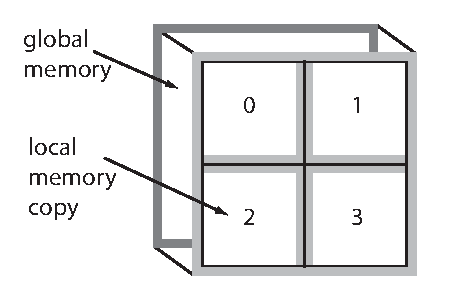
\includegraphics[width=1.75in]{cl-memory.pdf}
\caption{A schematic of global memory for an array and its copy stored in local memory
for four thread groups.}
\label{fig:cl-memory}
\end{figure}

We point out that the hierarchical distribution of memory used on the OpenCL
device shown in Figure~\ref{fig:cl-memory} is similar to the distribution of
memory across MPI nodes in an MPI application.  In the case of MPI, the
virtual global array is represented by the background layer (with its halo) and
partitions of the global array are stored in the 4 MPI nodes shown in the foreground.
Our current and future work on this effort includes source-to-source transformations
to generate MPI code in addition to OpenCL in order to deal with clusters of 
nodes containing accelerators.  This work is outside the scope of this paper.

Halo regions obtained via the {\tt region\_cpy} function (used with intent(in)
arrays) are constrained semantically so that they can not be written to by an
OpenCL kernel.  The {\tt region\_cpy} function returns a copy of the region of
the array stored in global memory and places it in local memory shared by
threads in a thread group.  Thus once memory for an array has been transferred
into global device memory by the host (before the OpenCL kernel is run), memory
is in a consistent state so that all kernel threads are free to read from global
device memory.  Because the local memory is a copy, it functions as a software
cache for the local thread group.  Thus the compiler must insert OpenCL barriers
at proper locations in the code to insure that all threads have written to the
local memory cache before any thread can start to read from the cache.  On exit
from a kernel, any local memory explicitly stored in register variables by the
compiler (memory accessed via the {\tt region\_cpy} function) is copied back to
global memory for all intent(out) arrays.  Recall that a thread may only write to
its own intent(out) array element, thus there are no race conditions when updating
intent(out) arrays.

%\subsection{ForOpenCL}

%This work describes transformations that automatically create OpenCL kernel
%functions from Fortran pure and elemental procedures.  At present, these transformations
%will not transform an entire program.  Users, for now, must explicitly replace
%calls to Fortran kernel procedures that run on the device, with calls to the
%OpenCL runtime that will run the kernel on the OpenCL host.  While these host
%transformations are straightforward using ROSE, they are outside the scope of
%this paper.

%In addition to the Fortran to OpenCL transformations, the
%ForOpenCL library available from the Open Fortran Parser web page provides programmers with the ability to
%call the C OpenCL runtime from Fortran.  ForOpenCL is a set of Fortran modules
%providing Fortran 2003 interface descriptions and classes that allow language
%interoperability with the OpenCL runtime.


\subsection{Transformation examples}

This section outlines the OpenCL equivalent syntax for portions of the Fortran
shallow-water code described in Section~\ref{sec:shallow-water}.  The notation
uses uppercase for arrays and lowercase for scalar quantities.  Variables
temporarily storing quantities for updated output arrays (declared as pointers
in Fortran) are denoted by a {\tt p} preceding the array name.  For example, the
Fortran statement {\tt pH = region\_ptr(oH, halo)} is transformed as a scalar
variable declaration representing a single element in the output array {\tt oH}.

\vskip .4in

\subsubsection{Region function}

While the Fortran version of the {\tt region\_cpy} function semantically returns
an array copy, in OpenCL this function returns a scalar quantity based on the
location of a thread in a thread group and the relationship of its location to
the array copy transferred to local memory.  Because we assume there is a thread
for every element in the interior, the array index is just the thread index
adjusted for the size of the halo.  Thus {\tt region\_cpy} is just an inline
OpenCL function and is provided by the ForOpenCL library.

\subsubsection{Function and variable declarations}

Fortran kernel procedures have direct correspondence with OpenCL equivalents.
For example, the {\tt wave\_advance} interface declaration is transformed as
{\small
\begin{verbatim}
__kernel void
wave_advance(float dx, ..., __global float * H, ...);
\end{verbatim}
}
\noindent
The intent(in) arrays have local equivalents that are stored in local memory
and are declared by, for example,
{\small
\begin{verbatim}
__local float H_local[LOCAL_SIZE];
\end{verbatim}
}
\noindent
These local arrays are declared with the appropriate size and are
copied to local memory by the compiler with an inlined library function.  The
array temporaries defined on cell faces are declared similarly while interior
pointer variables are simple scalars, e.g., {\tt float pH}.  Intent(in) array
variables cannot be scalar objects because regions may be shifted and thus
\emph{shared} by threads within a thread group.

\subsubsection{Array syntax}

Array syntax transforms nearly directly to OpenCL code.  For example, interior
pointer variables are particularly straightforward as they are scalar quantities in
OpenCL,
{\small
\begin{verbatim}
pH = region_cpy(H, halo)
       + (dt/dx) * ( region_cpy(Ux, face_lt) -
                     region_cpy(Ux, face_rt) )
       + (dt/dy) * ( region_cpy(Vy, face_dn) -
                     region_cpy(Vy, face_up) );
\end{verbatim}
}
\noindent
Allocated variables are more complicated because they are arrays.
{\small
\begin{verbatim}
Hx[i] = 0.5 * (region(H_local, face_lt)+ ...);
\end{verbatim}
}
\noindent
where {\tt i = LX + LY*(NLX+halo(0)+halo(1)))} is a local index variable, {\tt
  LX = get\_local\_id(0)} is the local thread id in the $x$ dimension, {\tt LY =
  get\_local\_id(1)} is the local thread id in the $y$ dimension, {\tt NLX =
  get\_local\_size(0)} is the size of the thread group in the $x$ dimension, and
the {\tt get\_local\_id} and {\tt get\_local\_size} functions are defined by the
OpenCL language standard.
